\documentclass[12pt]{report}
\usepackage{comment}
\usepackage{graphicx}
\usepackage{listings}
\usepackage{indentfirst}
\usepackage{setspace}
\usepackage{fullpage}
\usepackage{courier}
\usepackage[toc,page]{appendix}
\doublespacing
\usepackage{hyperref}
\usepackage{index}
\usepackage[nopostdot]{glossaries}
\makeglossaries

\newglossaryentry{ajax}{name={AJAX},description={Asynchronous JavaScript and XML. To quote from w3schools, ``AJAX allows web pages to be updated asynchronously by exchanging small amounts of data with the server behind the scenes. This means that it is possible to update parts of a web page, without reloading the whole page.'' For more information, visit \url{http://www.w3schools.com/ajax/ajax\_intro.asp}}}

\newglossaryentry{api}{name={API},description={Application Programming Interface. It defines and explains how users can use components of a program. A web's API usually guides users into permitted ways of extracting information from its database.}}

\newglossaryentry{bi}{name={Business Intelligence},description={technologies to congregate data for business analysis.}}

\newglossaryentry{crawl}{name={crawl},description={the process of downloading webpages and copy certain information from them.}}

\newglossaryentry{csv}{name={csv}, description={Comma-Separated Values, a plain text form of tabulated data. Entries in the same row are separated by commas,(sometimes pipelines or other characters) and columns are separated by newlines.}}

\newglossaryentry{json}{name={json}, description={JavaScript Object Notation, a human-readable format for storing data. It consists mostly of name/value pairs, so different parts of a data table will be easily recognized by their names.}}

\newglossaryentry{xml}{name={XML}, description={Extensible Markup Language, a markup language aiming to be both human-readable and machine-readable. It has tags illustrating the proceding values.}}

\newglossaryentry{harvest}{name={harvest}, description={Data Harvesting, the automated process of gathering and organizing data.}}

\newglossaryentry{mining}{name={Data Mining}, description={The practice of searching through large amounts of computerized data to find useful patterns or trends. (Definition from Merriam-Webster)}}

\newglossaryentry{ende}{name={encoding and decoding}, description={The conversion between elements of a certain language and numbers and texts. For instance, the character ``A'' is encoded as ``0X41'' in UTF-8 hex format, and ``01110001'' in UTF-8 binary format decodes to the character ``q''.}} 

\newglossaryentry{http}{name={HTTP Request},description={A message sent from the client to the server through actions such as clicking a button on a webpage, asking for information. The server will examine the message, and send a response message back to the client.}}

\newglossaryentry{xmlhttp}{name={XMLHTTPRequest},description={A JavaScript object. It provides an easy way to retrieve data from a URL without having to do a full page refresh,  allowing the response to be loaded within the script.\\(From \url{https://developer.mozilla.org/en-US/docs/Web/API/XMLHttpRequest}) }}

\newglossaryentry{js}{name={JavaScript}, description={A computer programming language that allows users to interact with contents on webpages.}}

\newglossaryentry{nlp}{name={NLP},description={Natural Language Processing, the study of using computers to interpret natural languages through linguistic analysis.}}

\newglossaryentry{nltk}{name={NLTK}, description={Natural Language ToolKit, a leading platform for building Python programs to work with human language data. It provides easy-to-use interfaces to over 50 corpora and lexical resources such as WordNet, along with a suite of text processing libraries for classification, tokenization, stemming, tagging, parsing, and semantic reasoning.(Extracted from \url{http://nltk.org/})}}

\begin{document}
\lstset{language=Python,
basicstyle=\ttfamily,
commentstyle=\textit,
breaklines=true,
numbersep=5pt,
xleftmargin=.25in,
xrightmargin=.25in,
columns=fullflexible,
showstringspaces=false}
\title{Web-Scraping:\\ How Charlotte Is A Life Saver Again}
\author{Fayang Pan}
\date{\today}
\maketitle
\tableofcontents
\listoffigures

\chapter{An Evaluation of Web-Scraping}
\section*{Introduction}

\indent Web-scraping is a way to collect existing information from the Internet. It is a nascent, powerful, but somewhat controversial subject in the arena of modern technology. Using tools to simulate viewing and downloading of a webpage through a browser, the `spider' (a metaphoric name for the part that goes into each web structure) goes into the webpage and `crawls' (a metaphor for copy-and-paste) desirable contents into a formatted data structure. Since this technology only requires access to the webpages, theoretically, anything that can be downloaded can be scraped off the Internet.

In the past summer, I worked with Pinnacle Solutions, Inc.,\footnote{For information, visit \url{http://psiconsultants.com/}} a company in Indianapolis, Indiana. My job was solely to develop web-scrapers. In this paper, I will provide an overview and discussion of web-scraping, followed by a description of my internship experience.

\section{An Overview of Web-Scraping}
In general, there are three basic ways to collect data: from primary sources, e.g., conducting surveys and studies; from compiled data in secondary sources, e.g., databases like the U.S. Census; and from existing but uncompiled information, e.g., product reviews from \textit{Amazon.com}. Web-scraping focuses on the last way: to \gls{harvest} data from a structured webpage, e.g., an HTML table, to a structured format, e.g., \gls{json} and \gls{csv}. It provides an amalgamation of the deluge of data spread over websites.

\section{Usage of Web-Scraping}
As web-scraping does not generate new data or results, it seems useless. However, people from various backgrounds may find web-scraping very useful. Here are a few examples:

If a student were to conduct a study on what lessons people learn from documentaries such as \textit{Food, Inc.}, he/she could go to \url{http://imdb.com}, \url{http://amazon.com} and \url{http://rottentomatoes.com} to scrape all the viewers' reviews. As there are thousands of reviews for the movie, web-scraping will help the student save much time trying to copy and paste every review. From the integrated results, the students might do a word frequency count to guess what kind of impression the majority have.

If a company were to have launched a product, they could use web-scraping to monitor their product, their competitors' products, and their partners' products. If people from Amazon.com  want to know how successful is the new Kindle Fire HDX, they can web-scrape all the reviews about Kindle Fire HDX, about Nexus 7, and about Kindle Fire HD. Through analysis, Amazon.com is able to collect customers' feedback promptly.

If a statistician were to monitor the price change of thousands of commodities, and if all these commodities are sold online, the statistician can use web-scraping to collect the prices. The scraper will just copy the prices from the product page of an online retailer website, and paste all of them into a spreadsheet. Shifts  in prices may reflect inflation/deflation, and the data can be used in economic research.

If a data analyst from Apple were to study how the public responds whenever a new product is released, he/she could collect the review dates from review websites and plot a frequency graph showing number of reviews per day. The number of reviews generated per day may reflect how receptive the customers are to a new product.

\section{Advantages of Web-Scraping}

\subsection{Speed}

Web-scraping allows people to copy and paste from webpages faster. For instance, someone wants to harvest 10,000 pieces of Amazon.com product reviews. Doing the job manually by copying and pasting every little piece of information into an excel spreadsheet would take a very long time and be prone to mistakes. Web-scraping technology, on the other hand, makes the process much faster. By specifying certain paths in the webpage structure, the spiders go into specific attributes and fields to \gls{crawl} information. With the help of web-scraping, 10,000 reviews can be copied and pasted into a \gls{csv} file within 15 minutes.\footnote{The result is based on running of my own scraper.}

\subsection{Convenience for Data Analysis}

Web-scraping improves the efficiency of data analysis. The tables of data that web-scraping produces are more easily processed than plain text. As web-scraping grabs from a structured format, it is able to copy and paste all the information needed into another structured format. For instance, after a \gls{csv} file is generated by scraping data from Amazon product reviews, all rows in the \textit{ratings} column have a range of 1 to 5 for number of stars, all rows in the \textit{review body} column will contain texts of the review bodies. A well-structured database will then provide foundation for further data \gls{mining} and other modeling techniques.

\subsection{Availability}

Web-scraping tools are becoming more widely available today. Popular tools for web-scraping include browser extensions such as \textit{firebug} and \textit{iMacros}, programs such as \textit{Wget}, programming languages such as \textit{Perl}, \textit{Hadoop} and \textit{Java} which have libraries to support sending HTTP requests, and programming language extensions such as \textit{Scrapy} and \textit{Beautiful Soup} for \textit{Python}. It is becoming more feasible for anyone to learn web-scraping, and to \gls{harvest} data beyond traditional methods such as using web \gls{api}.

\section{Challenges of Web-Scraping}

\subsection{Legality}

Web-scraping raises legal and ethical issues. While it is free to download many webpages, usage of the data within might not be in compliance with the terms and conditions of the source. 

There exists a fine line between using and stealing data. Currently, there is no law forbidding web-scraping all together, nor is there any way to ban downloading of webpages. However, as web-scraping becomes more versatile and powerful, companies are becoming more vigilant on data protection. 

In 2000, Bidder's Edge, a website that collects auction information from various websites, collected and displayed auction information from eBay. In response, eBay sued Bidder's Edge for ``trespass to chattels'',\footnote{For more information, visit \url{http://definitions.uslegal.com/t/trespass-to-chattels/}} and Bidder's Edge soon went out of business.\footnote{For information on the ruling, visit \url{http://www.tomwbell.com/NetLaw/Ch06/eBay.html}}

In March 2013, Associated Press (AP) won a lawsuit against Meltwater, a Norwegian group, over copyright infringement. Before the lawsuit, if a customer wanted to know how frequently a certain word appeared in the news, Meltwater could provide the information through scraping from various news websites. Meltwater used to be able to collect the news, put them into databases, and render them to customers on demand, but not any more. The court ruled that the usage of news resources went beyond the scope of ``fair usage'',\footnote{For more information about fair use, visit \url{http://fairuse.stanford.edu/overview/fair-use/four-factors/}} forbidding Meltwater from continuing to scrape from news agencies.\footnote{For more information on the ruling, visit \url{http://www.scribd.com/doc/131847330/Meltwater-AP-Ruling}}

In general, there are few things any scraper should watch out for. First, terms of use of the websites. Even though the terms are usually long and tedious, ``I did not see those'' is no excuse for violating the terms. Second, the scraper should also consider the purpose of the scraped information. If the scraper or customer were to use the scraped information for malicious purposes such as spamming and libel, it is likely to be illegal. Third, the scraper should consider the effect of scraping on others. If the number of requests for a certain scraping activity is too large for the website server to handle, other visitors to this website may experience malfunctions of the website. It is thus always wise to consult an attorney before beginning any commercial scraping activity.

\subsection{Intricate and Dynamic Web Structures}

In addition to legal concerns about scraping, prospective scrapers face increasingly complex web structures. \gls{ajax}, for instance, sends out an \gls{xmlhttp} only when the user performs certain maneuvers in the browser. Also, embedded \gls{js} contents may not be downloaded locally. The advent of these dynamic ways of loading web contents brings new challenges to web-scraping.

\subsection{Instability}
Another underlying problem comes from the fact that web-scraping is based on webpage structure. If the website adds a few toolbars, the locations of HTML attributes will change, resulting in a crash of the scraper. There also exists the problem of \gls{ende}. A scraper crash may also be caused by a website using unusual encoding of text. 

If the structure is dependent on a specific web browser, the content might appear different as well. A typical web-scraper downloads webpages with their HTML structures through the default browser, and a typical website offers the same HTML to any browser. However, some websites sometimes return different HTML structures to different web browsers for enhanced user experience, causing ambiguity of downloaded data. These potential problems manifest web-scraping's intrinsic dependence on the web interface.

In the following two pictures, the same webpage is opened using two different browsers, Google Chrome and Mozilla Firefox, under the same environment at the same time. Rendering of the page by the two browsers differ in locations of choice of flavor, availability of customer image, font sizes and layouts, sites available for sharing, etc.

\begin{figure}[htp]
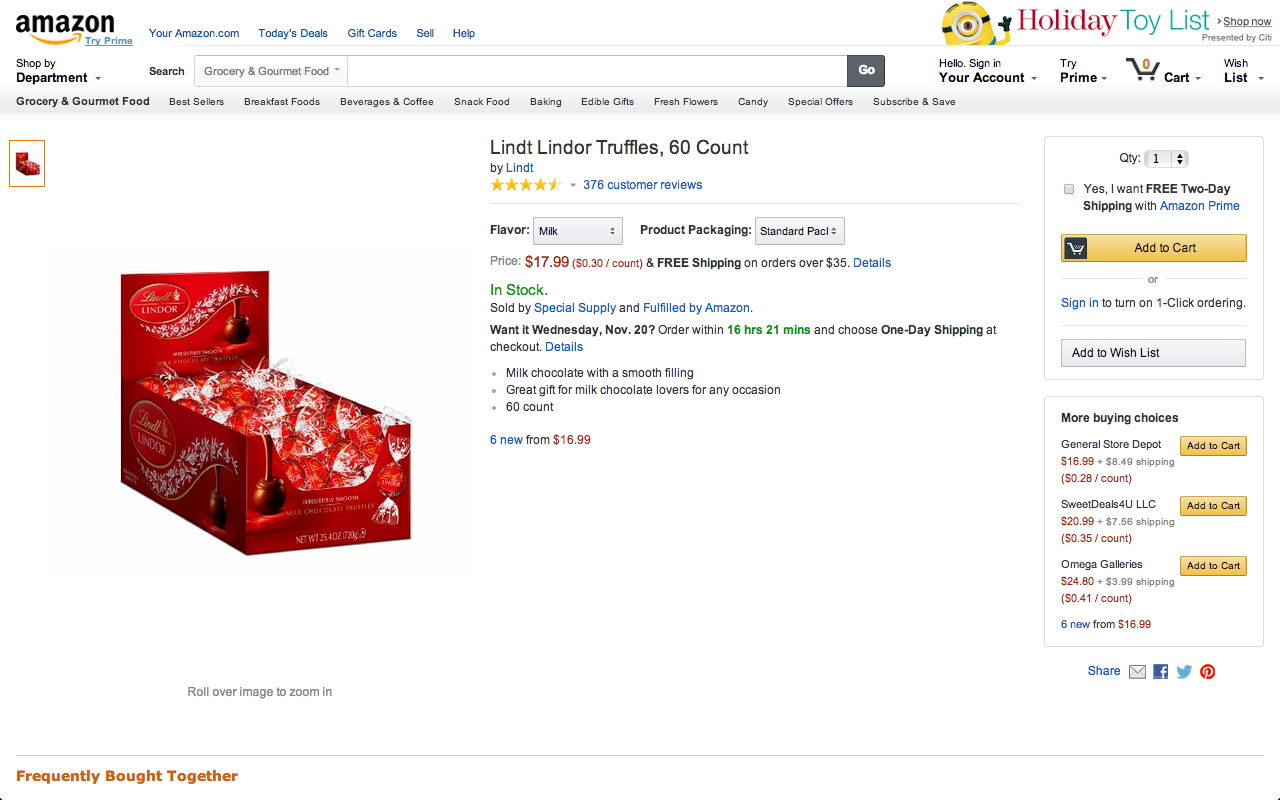
\includegraphics[width=\textwidth]{lindt_chrome.png}
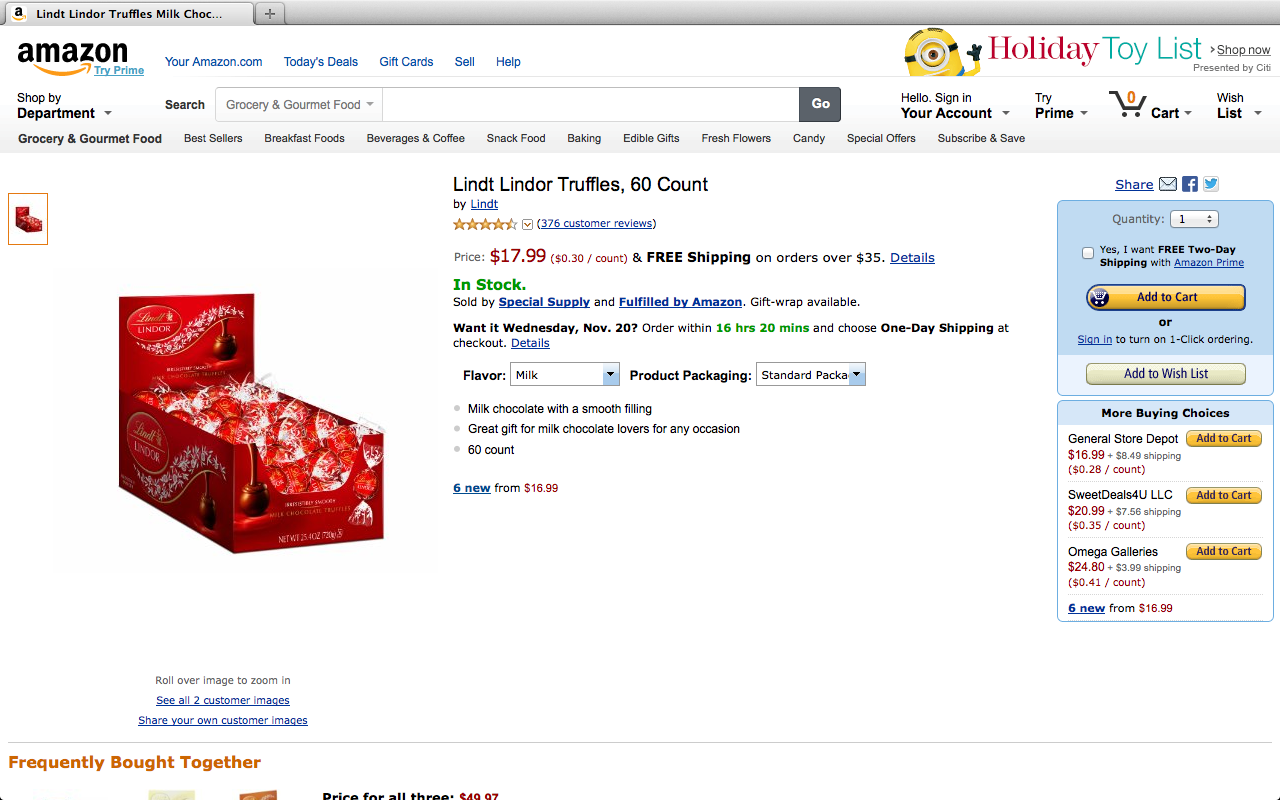
\includegraphics[width=\textwidth]{lindt_firefox.png}
\caption[Comparison of same url in different browsers]
{What Google Chrome displays versus what Firefox displays with identical urls.}
\end{figure}

\chapter{My Internship}
\section{Overview of My Internship at Pinnacle Solutions, Inc.}
Pinnacle Solutions, Inc.(PSI) is a start-up which helps clients to analyze and interpret their databases. Founded in 1996 by Kalamazoo College alumnus Donald Penix, Jr., the company, located in downtown Indianapolis, Indiana, currently has over 20 employees. PSI primarily uses \textit{SAS} for processing data, and \textit{Amazon Web Services} for server management.

I was a summer intern at PSI in 2011, and my job title was \gls{bi} Content Developer. At that time, Mr. Penix was very interested in sentiment analysis, a technology that aims to discover and analyze sentiment reflected through comments, reviews, and blog posts alike. For instance, a comment such as ``I love this iPad!" indicates a positive sentiment, and one such as ``I am sick of the iPad!" suggests a negative sentiment. Sentiment analysis will consolidate related comments and analyze them using \gls{mining} and \gls{nlp}. After research, we found sentiment analysis a tough job for PSI, as none of the employees had the needed expertise. So we decided to start from scratch, with data collection being the first step towards sentiment analysis.

\section{How Web-Scraping Became the Best Option}

Data analysis begins with data collection. As previously discussed, there are three ways to collect data. PSI is not interested in conducting primary research, because the research can be costly and lengthy. PSI would love to always have secondary databases available for analysis, but that is hardly possible, as PSI usually needs information beyond the scope of existing databases. Therefore, it becomes evident that PSI need to collect data from existing but uncompiled data from the Internet. Since large amount of data is needed, the process should be automated. In order to \gls{harvest} usable data from the Internet, there are many ways other than web-scraping.

First, one can extract necessary information using a web \gls{api}. Many websites offer APIs for developers to use to build applications. Twitter, for instance, published a new version of its API months ago. Through an API, users can request information directly from the website's databases, and the data will be clean and formatted. Twitter, for instance, offers exportable data in \gls{json} format. However, to obtain access to data in greater breadth, amount or detail, users may need to pay for them. Moreover, many websites may have limited information provided in their web APIs, or may not provide APIs at all. In that case, even though users can view the data from the browser, they cannot download it through APIs. Therefore, for a small company, it might be expensive and insufficient to rely on APIs for data harvesting.

Second, there are available third-party scraping and data harvesting services. There are applications like \textit{Mozenda},\footnote{\url{http://mozenda.com/}} and highly customizable services such as \textit{scrapinghub},\footnote{\url{http://scrapinghub.com/}} \textit{GNIP},\footnote{\url{http://gnip.com/}} and \textit{Open Amplify}.\footnote{\url{http://www.openamplify.com/}} However, these services are costly and, perhaps, beyond the means of small companies. Moreover, in the long run, as PSI needs more information from the Internet, its dependence on these services would be ever-increasing. Therefore, it would be a wise choice if PSI could come up with a low cost, independent system to harvest information. 

Third, as they are a certified \textit{SAS} reseller, they could use the software \textit{SAS Sentiment Analysis Studio}.\footnote{For more information, visit \url{http://www.sas.com/text-analytics/sentiment-analysis/}} However, this application is not only expensive for clients to buy, but also dependent on the web API. 

After many thorough discussion sessions, a free and open software solution capable of fetching data from the Internet via web-scraping was deemed desirable. Many web-scraping resources are free, so both the start-up and ongoing costs of doing web-scraping are low. There are many existing online communities discussing and developing web-scraping tools, so the technical support is active and extensive.

After some research, we chose Scrapy, a Python web-scraping framework, for the job.

\section{Scrapy, a Python Framework}

To quote from its website, ``Scrapy is a fast high-level screen scraping and web crawling framework, used to crawl websites and extract structured data from their pages. It can be used for a wide range of purposes, from data mining to monitoring and automated testing."\footnote{\url{http://scrapy.org/}}

Scrapy depends not only on Python, but also on a few other libraries. Scrapy uses Twisted,\footnote{\url{http://twistedmatrix.com/trac/}} an event-driven networking engine, and Zope,\footnote{\url{http://zope2.zope.org/about-zope-2/what-is-zope-2}} a web application server framework. The installation guide can be found on Scrapy's website.\footnote{\url{http://doc.scrapy.org/en/latest/intro/install.html}}

There are four basic classes in the Scrapy framework. These classes represent four main mechanisms of Scrapy. 

The spider. \textit{Spider.py} is responsible for downloading webpages, going into their structures and extracting data from them. At the very least, the user needs to specify the domain, the starting url, and the location in the webpage from which to crawl. If the user wants to scrape from multiple tables or multiple pages, or even conditionally scrape from certain pages, he/she can define those in \textit{Spider.py}.

The items. \textit{Items.py} is a class specifying the column names in the result. In the end, the result would be a table consisting of all the scraped data, and the items class defines what they are. Items in the same class will be in the same table.

The settings. \textit{Settings.py} includes instructions about what information will be written into the log file, limits on the frequency of requests sent, and other customizable features. In the event of a user login is needed, the user can pre-fill that in the login settings to avoid access denial.

The pipeline. \textit{Pipelines.py} decides how the scraped data are to be processed. By default, all data will be dumped into a single file. However, if the user wants to add a filter to remove some data, pipeline can handle that. If the user wants to split the results from one spider into two separate files, he/she can do that through coding in \textit{pipelines.py}.

Scrapy has more advanced features, which would fall outside of the scope of this paper. In the next chapter, I offer a high level approach to web-scraping using Scrapy.

\chapter{Scrapy Explained in Greater Detail}

\section{Test How Much You Can See}
Web-scraping depends on whatever the browser can "see," and there are times when the browser sees less than a person does. To check, one can use the following line of code in the command-line:\footnote{cmd.exe in Windows, Terminal in Mac OS/Linux} 
\begin{lstlisting}
scrapy shell http://amazon.com
\end{lstlisting}
After Scrapy finish analyzing the web address, it goes into its prompt and asks for further instructions. Here, the user can key in 
\begin{lstlisting}
view(response)
\end{lstlisting} 
A browser window opens and shows the structure of the website from Scrapy's perspective. The following two screenshots demonstrate the differences in downloading a page through Scrapy and viewing the page through the browser. 

\begin{figure}[htp]
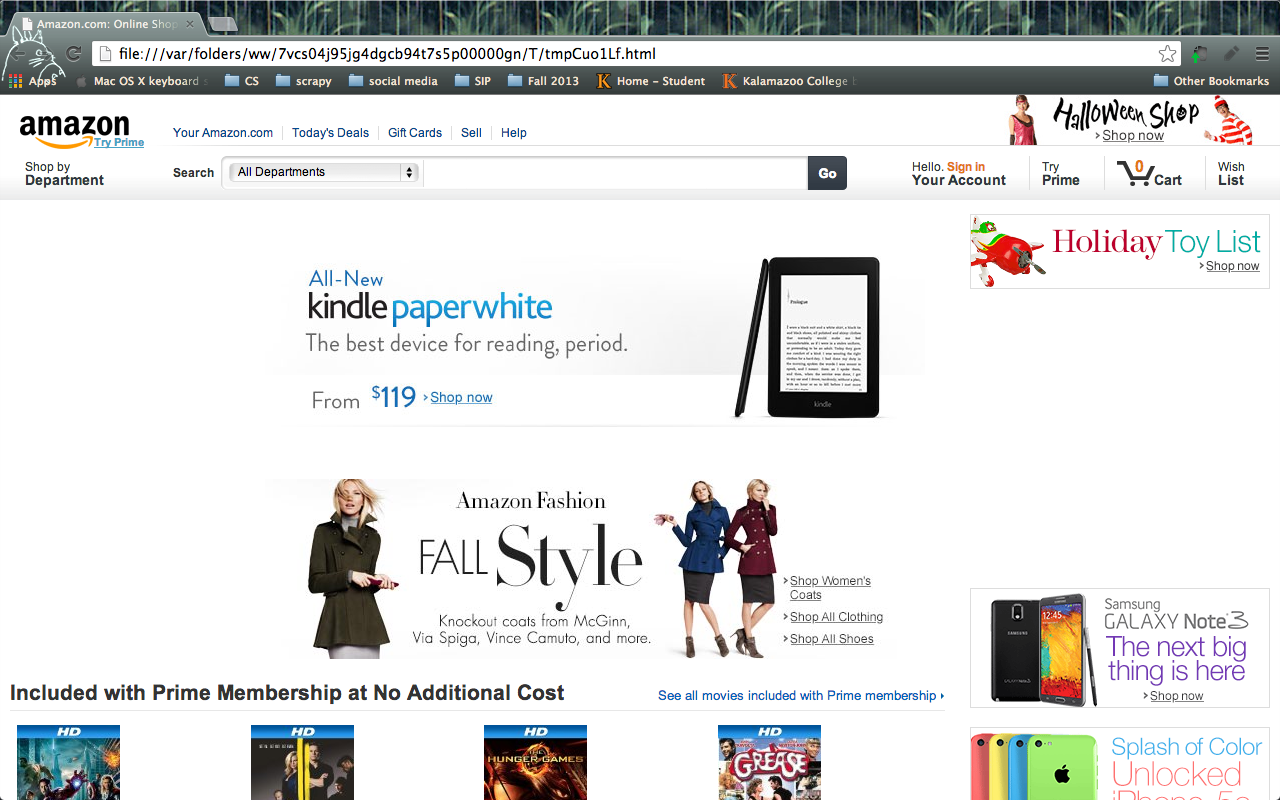
\includegraphics[width=\textwidth]{amazon_scrapy_view.png}
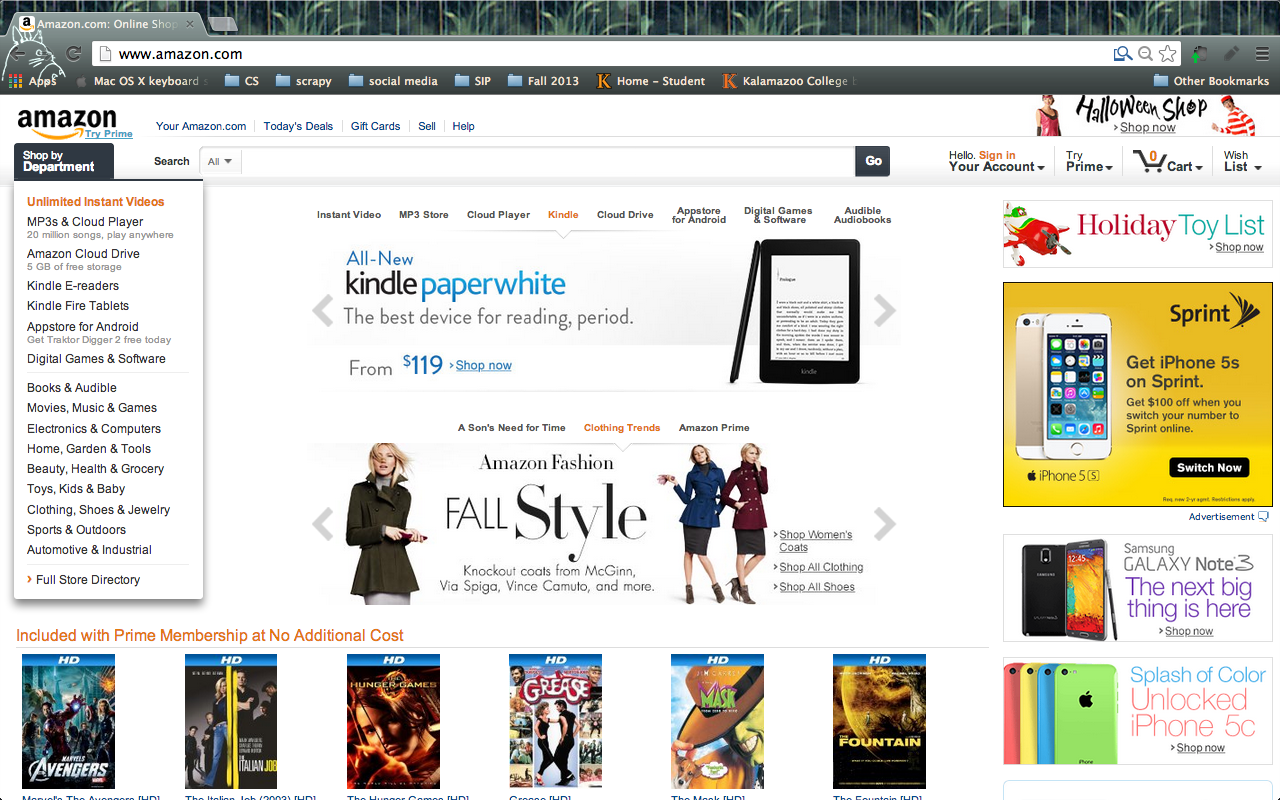
\includegraphics[width=\textwidth]{amazon_normal_view.png}
\caption[Comparison of views]
{What Scrapy is able to download locally (above) versus what the user can see (below).}
\end{figure}
\section{Test If the Data is Scrapable}
In theory, any data which can be seen can be downloaded, and any downloaded data can be scraped. In practice, however, it is not that simple. Even if Scrapy can see the data the user needs, the difficulty of scraping varies widely across websites. For instance, in the event of embedded \gls{js} code, scraping the result of a function call will be more difficult.

After setting up a project with few commands,\footnote{For more information, visit \url{http://doc.scrapy.org/en/latest/intro/tutorial.html}. The website has a simple example on how to start a project} it is wise to test if certain data are scrapable. Before knowing if the data are scrapable, one needs to specify where exactly the data are located. To establish a standard way of referring to a certain field in the webpage, XPath\footnote{Abbreviation of ``XML Path Language''.For more information, see \url{http://www.w3.org/TR/xpath/}}is used.

To retrieve a certain XPath, one can use a built-in \textit{``Inspect Element''} tool, or an extension such as \textit{firebug},\footnote{Visit \url{http://getfirebug.com/ for more information}} available for \textit{Firefox} and \textit{Google Chrome}. Figure 3.2 provides an example using \textit{``Inspect Element''} in \textit{Google Chrome} to extract an XPath from \url{http://www.nbcnews.com}.\\
\begin{figure}[htp]
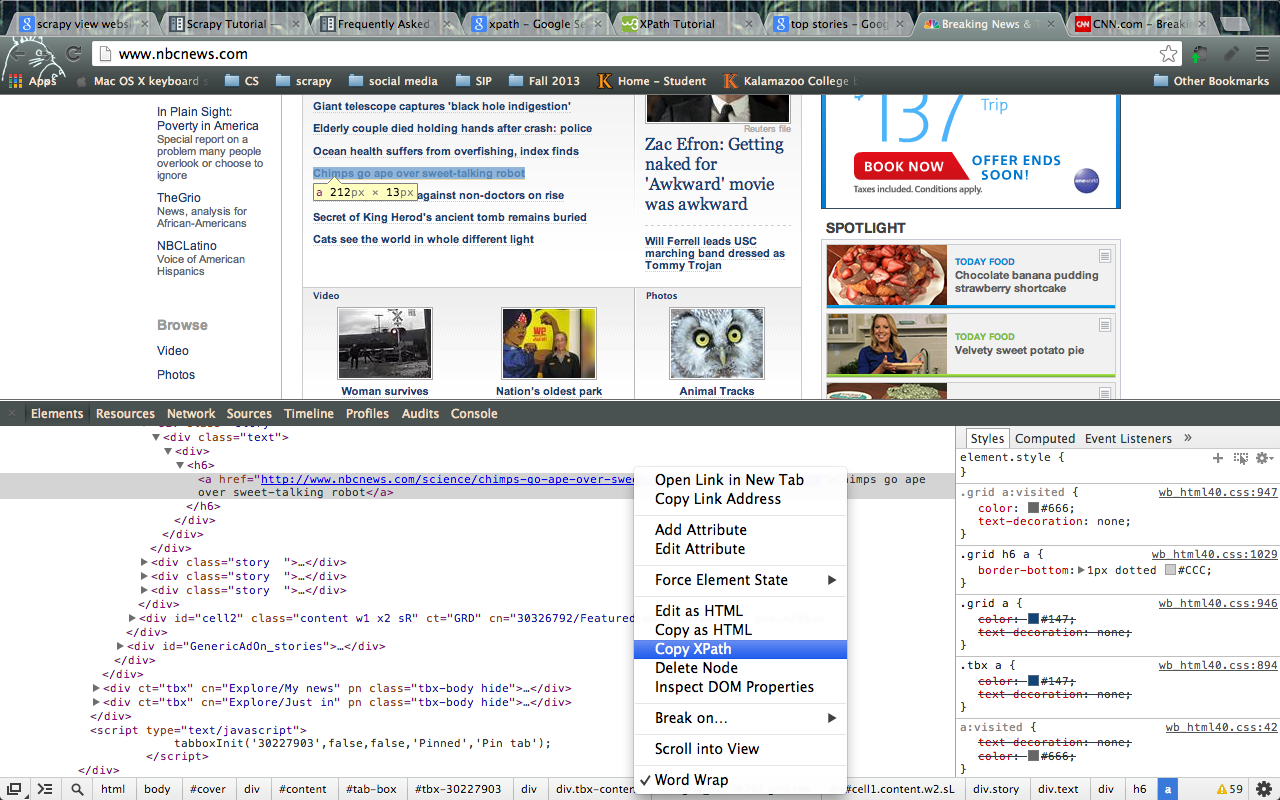
\includegraphics[width=\textwidth]{XPath_example.png}
\caption[How to extract XPath]
{A screenshot of how to obtain an XPath from a webpage, and the XPath of the link is \textit{//*[@id=``cell1'']/div[8]/div/div/h6/a}.}
\end{figure}
Given a specific XPath, one can write related code to test if Scrapy can recognize the XPath and scrape the data. If one piece of data is scrapable, it is likely that the entire table which contains that piece of data can be scraped. If the sample table is scrapable, it is also likely that similar tables can be scraped, too.
\newpage
\section{Iterators}

Web-scraping relies heavily on the structure of the webpage. If the webpage is very organized, it is possible for the user to use XPath to find all entries in a table, and send out a request to scrape the next page. In Scrapy, the request is in the form of a callback function. The spider will scrape the data, yield the results from the page, and then excute the callback function. Here is a snippet of that concept:
\begin{lstlisting}
class Spider(BaseSpider):
	def parse(self,response):
	##some code to extract data from this current page
		yield results_from_this_page
		if next_page:
			yield Request(url_of_the_next_page,callback=self.parse)
\end{lstlisting}

In the code above, \textit{BaseSpider} is one of the spider classes the user has to inherit to build a user-defined spider. In any spider class, a method like \textit{parse(self,response)} is necessary to communicate with the computer and instruct which fields in the html to scrape from. The \textit{parse} method yields a generator, but the code does not necessarily end there. In the event that there is a next page with the same html format, the parse method will be able to go into the new html webpage and collect the new data in the same way it did for the previous page. Therefore, the method \textit{parse} can also yield a \textit{Request}. \textit{Request} represents an \gls{http} in many cases. It sends a signal to the scraper and asks for a \textit{Response}, which will be handed to the spider and the spider will scrape it.

\section{Specification}

After sketching and testing the basic functionalities, we proceed to consider the types of information clients want and the types of information needed to make database management easier. 

The clients usually ask for specific data that are useful to their businesses. For instance, an author may want to read all of the reviewers of her latest book. To collect book reviews from websites such as \url{http://amazon.com} and \url{http://goodreads.com}, we need different spiders, one for each website. Nevertheless, it may be possible to instruct the spiders to generate tables with identical column names so that the author can view everything in one sheet. That data sheet may contain book name, edition number, publisher, review website, user name of the reviewer, date of review, ratings, review bodies, and other information as the column names.

On the developer's end, however, the structure will be very different. To track every piece of review, the developer may need a column with the url from which that particular review was pulled. To establish an iterator, the developer may need to track the book identification number on the website to generate the correct url to scrape from. To deal with different encodings and web structures of different websites, the developer needs to customize every spider.

A piece of pseudo-code for extracting a certain text could be:
\begin{lstlisting}
item['some_field']=HtmlXPathSelector(response).select('SOME/XPATH/IN/HTML/text()').extract()
\end{lstlisting}

\section{Produce a sample output}

After studying what and how the spider should scrape from webpages, we are ready to produce a sample output. The sample output is necessary for three reasons.

First, formatting and encoding. It is not unusual when the ideal is far from reality. Although XPath offers a specific location of all scrapable information, it is highly possible that the formatting is not desirable. Also, most websites are written in utf-8, but Python's csv module defaults encoding to ascii, a paragraph often has a \textit{\textbackslash u} in front of it. For instance, a review ``I like this!'' will be translated into \textbackslash u``   ,    ,    ,   , I like this!'' through Scrapy.
\begin{figure}[htp]
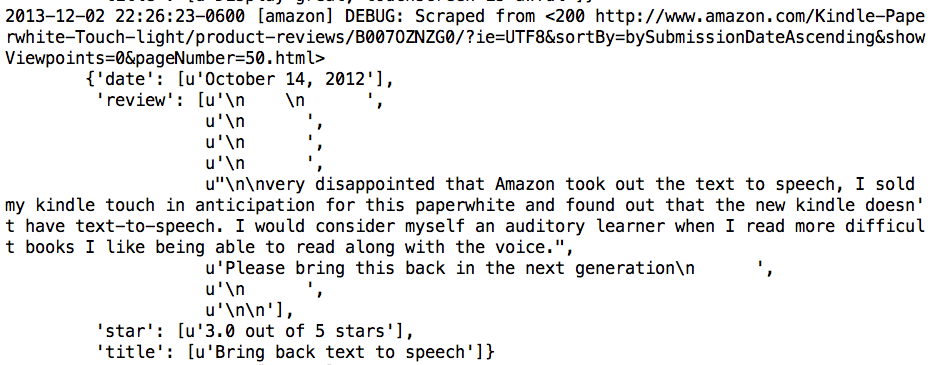
\includegraphics[width=\textwidth]{scrapy_screenshot_terminal.png}
\caption[Scrapy screenshot in Mac Terminal]
{What extracted data may look like in Terminal.}
\end{figure}

Second, communication with clients and manager. Only when the sample data sheet is out, can the results of scraping be evaluated. There are limitations to scraping, so it is essential to make clients and managers aware of those. For instance, the time of producing a sample output influences the frequency of running the scraper. In the event that the target website restricts IP address from visiting it too fast, the time taken to scrape data will definitely be longer than expected.

Third, testing. As web-scraping is based on web structure and HTTP requests, it is unstable by nature. Although the code may work perfectly in theory, it may encounter problems in practice. These problem may be relevant to Internet connection, broadband width, geographic location, configuration of the computer, and other factors which may influence the scraping process. As the spider sends out requests and receive responses at a fast pace, it might encounter concurrency issues, causing some data to be skipped over or scraped repeatedly. All these issues are instrumental to the performance of a certain spider and Scrapy project, so the developer needs to read the sample output in great detail and make amendments on the code.
\begin{figure}[htp]
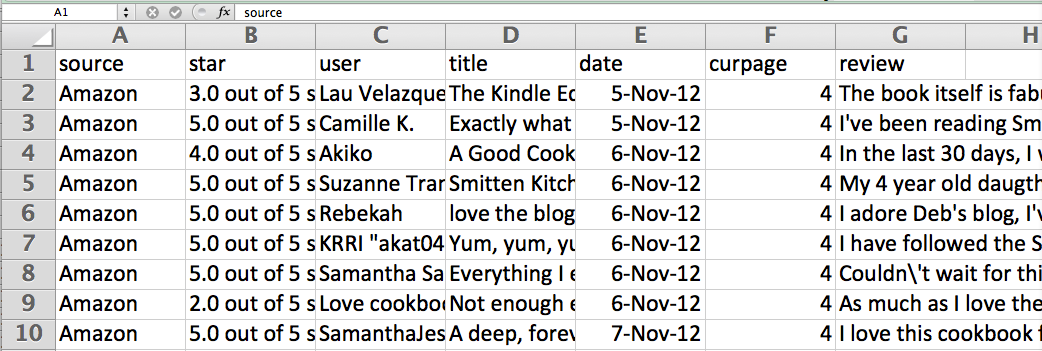
\includegraphics[width=\textwidth]{sample_output.png}
\caption[Sample csv output]
{What extracted data may look like in csv format.}
\end{figure}

After the sample output seems qualified, the developer may consider other functionalities which may enhance the utility of a particular scraper. 

For instance, to efficiently scrape updated reviews from a website, one can build a last page tracker. If a product has 50 pages of reviews on day 1, one can view the reviews by ascending date order so that the latest review appears on the last page. After the scraper scrapes the 50 pages on day 1, it store the last page as 50, so that when there are 60 pages on day 2, the scraper can start scraping from page 50 to 60, without re-scraping the first 49 pages.

For another instance, one can make the scraper more interactive with the user. One can use Pipeline to save the output data into a user specified directory. For some scraping job like product reviews, it is also possible to ask for an identifier of the product, and the scraping process will start from an auto-generated url.

\chapter{Future Development of the Project}


\section{Natural Language Toolkit}
After harvesting data from online sources, there are various ways to enjoy the fruit. This chapter will illustrate some of possible ways to use the data.

Natural Language ToolKit, or \gls{nltk}, has many functions, and one of them is tokenization. Tokenization is the process of breaking up a paragraph into sentences, a sentence into phrases, a phrase to words, or even a word to its components. These subsets are called tokens, and more study can be done through analyzing these tokens.

For instance, if a product manager would like to monitor the sentiment of customers on the product, he/she could use web-scraping to collect review texts from online rating websites. Although those texts are available, the feedback from the reviews are not quantitative. With \gls{nltk}, however, one can tokenize each review into sentences, and sentences into phrases. For example, one can assign a score of ``1'' if the review says ``I hate this product!'', and a score of ``10'' if the review reads ``I love this product!''. There are databases such as WordNet available for download as a package for \gls{nltk}, and there are algorithms for assigning scores to words.

However, there are few challenges in the process of detecting sentiment. 

First, the ambiguity of language. Same word may have different meanings in different context. For instance, in the review of a product, ``I am sick of it'' and ``This product is sick!'' have opposite sentiments, but they both use the word ``sick'' to express the sentiment. As the internet language becomes increasingly versatile, with slangs, emoticons, puns, and other forms of language in the scraped text, the difficulty of guessing the right sentiment of an expression increases drastically.

Second, the complexity of language. Short statements such as ``This product is great!'' and ``I hate it!'' are generally easier for sentiment detection. As the statement becomes longer into a complex sentence, a paragraph or even multiple paragraphs, the evaluation of a certain review becomes more complicated, too. For instance, for a review such as ``Though this product may not be the worst in the world, please choose other products if possible.'', it seems obvious to human that the sentence contains negative sentiment against the product. To the computer, however, when it sees ``not'' followed by ``worst'', it may assign a very positive sentiment to this review.

\section{Data Mining}

Web-scraping has the potential of collecting data from multiple facets. When a review website displays reviews on its webpage, information such as date, ratings, review texts and other relevant details will be available as well. 

While it seems feasible to operate data mining under many collectable variables, the actual practice will not be easy. There are two main limitations.

First, limitation of parsing. The default format of scraped data is string, but more often than not, numbers are preferred in data mining. The process of parsing numbers from their string representations may incur errors.

Second, limitation of accessible data. Websites are not likely to display some data, such as demographic data, to the public. To investigate possible correlations, insufficient data will be available for scraping.


\section{Graphic User Interface}

For future development of web-scraping, it is possible to build an user interface from the code. 

To scrape information related to a particular item, the user can choose a website to scrape from, and input necessary fields such as the unique identifier of that item in the website. Then, the user can choose from a checklist of what areas to scrape from, and the number of results shown. Then, after clicking a button, the Python script at the back end will use Scrapy to retrieve the input information, create starting and ending urls, and scrape selected results from relevant pages.

However, there are few limitations of establishing an interface.

First, validity of user input. As the back end Python script retrieves information from the user interface, invalid input may cause the program to stop functioning.

Second, constantly changing web interfaces. As web-scraping depends heavily on web structures, in the event of a change in web interfaces, the spider will probably fail to crawl information. Therefore, both the programmer and the user need to update frequently. The stability of the software will be very fragile.

\newpage
\begin{appendices}
\printglossaries
\end{appendices}
\end{document}
